\documentclass[12pt]{article}
\usepackage[english]{babel}
% \usepackage[utf8x]{inputenc}
\usepackage[T1]{fontenc}
\usepackage{scribe}
\usepackage{listings}
\usepackage{fullpage}
\usepackage{amsfonts}
\usepackage{amssymb}
\usepackage{hyperref}
\usepackage{url}
\usepackage[svgnames]{xcolor}
\usepackage{color}
% \definecolor{light-gray}{gray}{0.90}
% \lstset{backgroundcolor=\color{light-gray},showlines=true}

% \usepackage{xcolor}
% \usepackage{listings}

% \lstdefinestyle{BashInputStyle}{
%   language=bash,
%   basicstyle=\small\sffamily,
%   numbers=left,
%   numberstyle=\tiny,
%   numbersep=3pt,
%   frame=tb,
%   columns=fullflexible,
%   backgroundcolor=\color{yellow!20},
%   linewidth=0.9\linewidth,
%   xleftmargin=0.1\linewidth
% }


\usepackage{minted}
\setminted{fontsize=\footnotesize,baselinestretch=0.5}



\Scribe{}
\Lecturer{Queenie Qiu, John Raiti. Student: \textbf{Shucheng Guo}}
\LectureNumber{5}
\LectureDate{DATE: Feb 16th. 2023}
\LectureTitle{Introduction to Robotic Arm Kinematics}

\lstset{style=mystyle}

\begin{document}
	\MakeScribeTop

%#############################################################
%#############################################################
%#############################################################
%#############################################################

\section{Learning Objectives}
\begin{enumerate}
    \item Learn the difference between arm motions in task-space and configuration-space.
    
    \item Familiarize yourself with MoveIt! as a ROS component.
    
    \item Implement high-level nodes through MoveIt! combined with RViz and Gazebo to move a Kinova Gen3lite arm and a Fetch robotics arm using forward and inverse kinematics.
\end{enumerate}


\section{Introducing Kinova Gen3lite
}
\subsection{ROS Kortex Package Installation}
ROS Kortex is the official ROS package to interact with Kortex and its related products. These are the instructions to run in a terminal to clone the ros\_kortex repository and install the necessary ROS dependencies. \\
\textbf{Note}:The default branch for git clone is developed for ROS Noetic. If you are using other ROS distributions, please git clone to corresponding branch.
\begin{minted}{bash}
    $ sudo apt install python3 python3-pip
    $ sudo python3 -m pip install conan
    $ conan config set general.revisions_enabled=1
    $ conan profile new default --detect > /dev/null
    $ conan profile update settings.compiler.libcxx=libstdc++11 default
    $ cd catkin_ws/src
    $ git clone https://github.com/Kinovarobotics/ros_kortex.git
    $ cd ../
    $ rosdep install --from-paths src --ignore-src -y
    \end{minted}
Then, to build and source the workspace:
\begin{minted}{bash}
    $ catkin_make
    $ source devel/setup.bash
    \end{minted}

\subsection{Spawning a Kinova Gen3lite robot in Gazebo}

We will use the ros\_kortex repository to work with the Kinova arm. In this metapackage, we will use the kortex\_gazebo portion for simulation. Execute the following launch file that will bring up a gen3lite in Gazebo and open an RViZ window
\begin{minted}{bash}
    $ roslaunch kortex_gazebo spawn_kortex_robot.launch arm:=gen3_lite z0:=0.8
    \end{minted}

The Gazebo window looks like:

\begin{figure}[H]
    \vspace{-10pt}
    \centering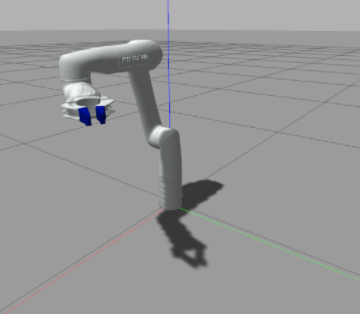
\includegraphics[width=5cm]{images/gazebo.PNG}\vspace{-10pt}
    \caption{Spawning in Gazebo.}\label{fig:gazebo}
    \end{figure}

Note: Once the RViZ and Gazebo windows have been opened, and the terminal shows two green messages ( “You can start planning now!” and “The Kortex driver has been initialized correctly!” ) you can add a Robot model and add a MotionPlanning component in Rviz.

\begin{figure}[H]
    \vspace{-10pt}
    \centering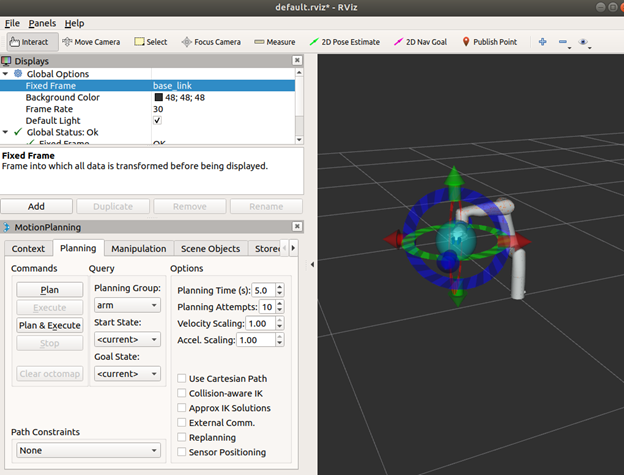
\includegraphics[width=10cm]{images/rviz1.png}\vspace{-10pt}
    \caption{Kinova arm in Rviz.}\label{fig:rviz1}
    \end{figure}

\subsection{Using the Interactive Markers to change the robot’s pose based on the task-space}


You can use the different arrows and rings on the interactive marker, to change positions and orientations of the robot’s end-effector. As you use them, you will see an orange version of the robot arm with the proposed new position. Once you have reached a desired position, use the buttons “Plan” and “Execute”(in the MotionPlanning Panel) to make the robot in Gazebo move to the new proposed position. Some useful tools for you to track the robot’s motions are:

\begin{enumerate}
    \item Check the values of the joints:
        \begin{minted}{bash}
        $ rostopic echo -n 1 /my_gen3_lite/joint_states
        \end{minted}
    \item Outputs the pose of the robot’s end-effector with respect to the world (in this case Gazebo’s origin):

        \begin{minted}{bash}
        $ rosrun tf tf_echo /world /end_effector_link
        \end{minted}

    \item You may also consider using the base link as the reference:
        \begin{minted}{bash}
        $ rosrun tf tf_echo /base_link <END-EFFECTOR LINK>
        \end{minted}
\end{enumerate}    
If you want to change the state of the gripper, you need to change the Planning Group (in the MotionPlanning Panel) from arm to gripper, and you can select a new position.
\\

\textbf{Deliverables:}
\begin{enumerate}
    \item Add a TF component in RViz and enable only the base\_link and the end\_effector\_link. Disable the Motion Planning component to temporarily remove the interactive markers. Add a screenshot of the RViZ view.
    
    \begin{figure}[h]
        \centering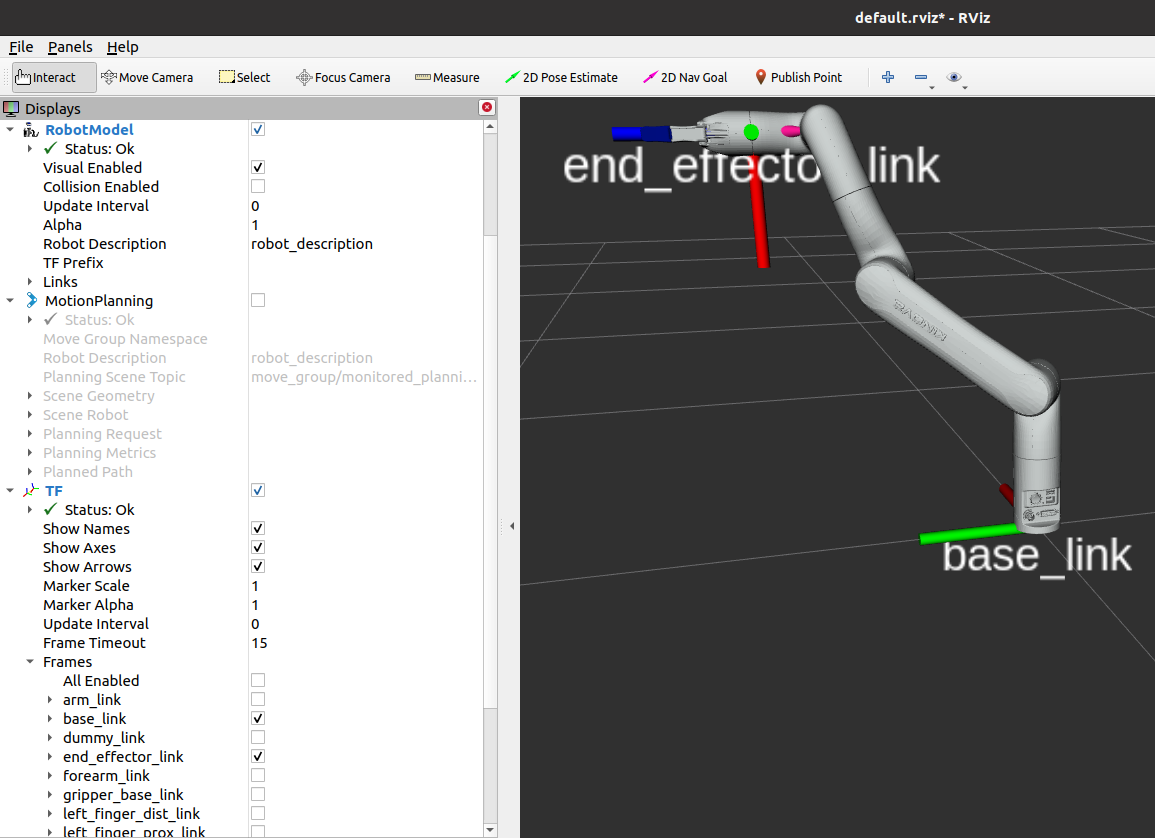
\includegraphics[width=14cm]{images/kinova_rviz.png}\vspace{-4pt}
        \caption{RViZ with Kinova.}\label{fig:kinova_rviz}
        \end{figure}

    \item Use rqt\_tf\_tree to determine the kinematic chain between the two reference frames (base\_link and end\_effector\_link).
    
    \item Turn on the Motion Planning component again. The "Goal State" in the MotionPlanning panel allows you to set goals to some predefined positions. Inspect it and report what are the reported robot’s joints values and pose (wrt the world) when you send the gen3lite to the following preset positions:\\
    a. Home\\
    b. Retract\\
    c. Select a robot pose that you would choose if you had to pick something from the table. Add a screenshot of the resulting pose of the arm in \textbf{Gazebo}.
\end{enumerate}

\subsection{Using the Joints tab in MotionPlanning to change the robot’s pose on the configuration-space}

In the MotionPlanning panel, find the "Joints" tab. You will be able to change the values of the different joint angles. Explore the configuration space, determine which joints move in which direction when a positive or a negative angle is given to each joint.
\\

\textbf{Deliverables:}
\begin{enumerate}
    \item Configure the joint angles and move to your desired position. Add a screenshot of the rviz window(including joint values and the robot visualization), use the same tools described in the previous subsection to explore the values for the pose and the joint angles.
    
    \item Explain the differences you observed when controlling the robot’s position using either the interactive markers or the joint angles.
    
    \item Can you change all joint angles from the RViZ window? If not, explain what degree of freedom is not available and how that impacts the poses you can reach with the robot.
\end{enumerate}


\section{Introducing Fetch Robot}
\subsection{Fetch Packages Installation}
Following the instructions to install packages from from Fetch Robotics.
\begin{minted}{bash}
    $ cd catkin_ws/src
    $ git clone -b ros1 https://github.com/fetchrobotics/fetch_ros.git
    $ git clone -b gazebo11 https://github.com/fetchrobotics/fetch_gazebo.git
    $ git clone -b ros1 https://github.com/fetchrobotics/fetch_msgs.git
    $ git clone -b ros1 https://github.com/fetchrobotics/power_msgs.git
    $ git clone -b ros1 https://github.com/fetchrobotics/robot_controllers.git
    $ cd ../
    $ rosdep install --from-paths src --ignore-src -y
    (Ignore the error: Unable to locate package ros-noetic-simple-grasping)
    $ sudo apt install ros-noetic-rgbd-launch
    \end{minted}
\textbf{Note}:The branch "ros1" and "gazebo11" is developed for ROS Noetic. If you are using other ROS distributions, please git clone to corresponding branch.
\subsection{Fetch Robot Manipulation}
We will go through a similar procedure as the Kinova Gen3lite, familiarizing ourselves with the arm components of the Fetch robot. Execute the following commands in different terminals to spawn a Gazebo simulated Fetch robot, activate the motion capabilities and open an RViZ window

\begin{minted}{bash}
    $ roslaunch fetch_gazebo simulation.launch
    $ roslaunch fetch_moveit_config move_group.launch
    $ rosrun rviz rviz
    \end{minted}

You will need to add the Robot Model and the MotionPlanning components in RViZ once it opens. Check the rqt\_tf\_tree to determine the name of the end-effector’s link to run the command:

\begin{minted}{bash}
    $ rosrun tf tf_echo /odom <END-EFFECTOR LINK>
    \end{minted}
    
You may also consider using the start of the arm chain as the reference:

\begin{minted}{bash}
    $ rosrun tf tf_echo /<FIRST ARM JOINT> <END-EFFECTOR LINK>
    \end{minted}

\begin{figure}[H]
    \vspace{-10pt}
    \centering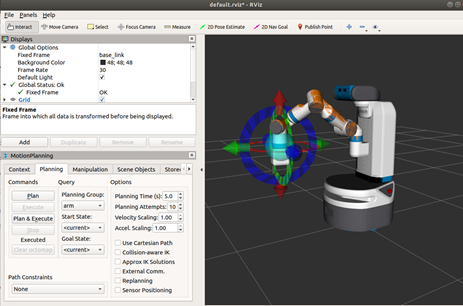
\includegraphics[width=10cm]{images/rviz2.png}\vspace{-10pt}
    \caption{Fetch in Rviz.}\label{fig:rviz2}
    \end{figure}

\textbf{Deliverables:}
\begin{enumerate}
    \item Add a TF component in RViz and enable only the base\_link, the first joint of the arm, and the end\_effector\_link. Disable the Motion Planning component to remove temporarily the interactive markers. Add a screenshot of the RViZ view.

    % \begin{figure}[h]
    %     \centering\includegraphics[width=14cm]{images/fetch_rviz.png}\vspace{-4pt}
    %     \caption{RViZ with Fetch.}\label{fig:fetch_rviz}
    %     \end{figure}
    
    \item Use rqt\_tf\_tree to determine the kinematic chain between the two reference frames.
    
    \item Unlike the Kinova arm, the MotionPlanning for Fetch does not have preset poses for the arm.
    \begin{enumerate}
        \item Show a screenshot of the resulting pose when all joints in the arm are set to 0 degrees.
        \item Report the joint angle values of all Fetch’s arm joints on a pose that would allow Fetch to pick up an object from the floor.
    \end{enumerate}
    
    \item Explain the differences you observed when controlling the robot’s position using either the interactive markers or the joint angles.
    \item Can you change all joint angles from the RViZ window? If not, explain what degree of freedom is not available and how that impacts the poses you can reach with the robot.
\end{enumerate}

\section{Using Python to control Fetch robots}

Now that we have familiarized the robot, we will create nodes that will generate motions on Fetch robot. One will move the robot arm by assigning values to joints angle, applying \textbf{forward kinematics} to reach to the target position and orientation of the end-effector in Cartesian space. Another node will apply 
\textbf{inverse kinematics} which calculate and change the joint angles based on the given target pose of the end-effector. You will use working code provided on canvas as a guide. You may need to modify the code to finish the deliverable.

\textbf{Notes:}
You can visit the Fetch documentation for \href{https://docs.fetchrobotics.com/manipulation.html#running-the-pick-and-place-demo}{additional tutorials}. \\

\textbf{Deliverables:}
\begin{enumerate}
    \item Please identify which Python file corresponds to each type of robot kinematics?
    
    \item Capture videos of the robot executing movements using both programs, separately. Upload them to Canvas with your writeup. 
    
    \item Modify the code that performs forward kinematics and move the arm to a pose with your desired input values. Compare the resulting angle values (rostopic echo /joint\_states) to your inputs.

    \item Modify the code that performs inverse kinematics and move the arm to a pose with your desired input values. Then compare the resulting pose (rosrun tf tf\_echo /<link1> /<link2) to your inputs.
    
    \item Discuss what type of robot kinematics was faster to use? Which one was easier to use?
    
    \item What were the advantages and disadvantages of using RViz or generated code to control the robot's motion? Please provide at least two thoughts.
\end{enumerate}


\end{document}